\documentclass[letterpaper,twoside,onecolumn,openright,final]{memoir}
%    vs.       others...   oneside twocolumn openleft  draft showtrims
%                          twoside onecolumn openany   ms
%                                            openright final 
\input lumos_common
\begin{document}
\frontmatter

\thispagestyle{empty}
\ThisLLCornerWallPaper{1}{images/4cover}
%\strut
\vfill
\begin{center}
{\fontfamily{ppl}\fontseries{b}\fontsize{48}{50}\selectfont
\strut Installing the \\\strut Lumos\TM\\\strut
4-Channel \\\strut DC Controller}

\vfill

\end{center}

\newpage
\begin{center}
\LLimg[width=1in]{danger-generic}

%DANGER! 

\mc{RISK OF FIRE, ELECTROCUTION, SERIOUS INJURY OR DEATH!} 
\end{center}

This circuit design, including but not limited to any associated plans, schematics, designs, board layouts, documentation, 
and/or components, is \mc{EXPERIMENTAL} and for \mc{EDUCATIONAL} purposes only. It is not a finished consumer-grade product.
It is assumed that you have the necessary understanding and skill to assemble and/or use electronic circuits.

Proceed \mc{ONLY} if you know exactly what you are doing, understand the proper procedures for working with the high voltage present on the components and PC boards, and understand that you do so \mc{ENTIRELY AT YOUR OWN RISK.}

The author makes \mc{NO} representation as to suitability or fitness for any purpose whatsoever, and disclaims any and all liability or warranty to the full extent permitted by applicable law.
\index{warranty, limitation of}
\index{danger warnings}
\index{warnings}

\strut\vfill
\noindent Edition 1.0, for Lumos 4-Channel DC Controller circuit version 1.0.

\smallskip


\noindent Copyright \copyright\ 2014 by Steven L. Willoughby,
Aloha, Oregon, USA.  All Rights Reserved.  
This document is released under the terms and conditions of the 
Creative Commons ``Attribution-NoDerivs 3.0 Unported'' license.  
In summary, you are free to use, reproduce, and redistribute this 
document provided you give full attribution to its author and do not
alter it or create derivative works from it.  See
\URL{http://creativecommons.org/licenses/by\-nd\-/\-3.0/} for the full
set of licensing terms.

\begin{center}
\LLimg[width=.5in]{cc}\LLimg[width=.5in]{by}\LLimg[width=.5in]{nd}
\end{center}

\newpage
\tableofcontents
\listoffigures

\mainmatter

\chapter{Introduction}
\LLstart{C}{ongratulations}{on joining} the many computer-controlled
Christmas light enthusiasts, \ix{theatrical lighting} technicians, electronics hobbyists,
\index{Christmas lights}
and home automation innovators who are experimenting with new ways to have computers
control lights and other electronic devices.

The Lumos\TM\ 4-Channel DC Controller board places four such devices under the control
of your computer.  These outputs are 
electrically isolated from the logic control circuit (although you may opt to forego that
isolation and power the logic and loads from the same supply).

Since these Lumos boards use \acronym{RS-485} for communications, up to sixteen Lumos
boards may be ``daisy chained'' together and controlled from 
the same PC serial port.
By plugging DC-powered Christmas lights into the Lumos controller, your PC can orchestrate
a dazzling display of lights synchronized to music.

This manual assumes you have a Lumos controller board built and ready to put into operation.
We will describe how to install it in a working circuit.  

The operational details involved
in getting the controller to work with software is described in 
\emph{Using Lumos\TM\ SSR Controllers.}

\section{Intended Audience}
This is an ``advanced'' level do-it-yourself electronic circuit project.  It is not
an off-the-shelf consumer-ready product.  It is only designed for educational and experimental
use by experienced hobbyists and professionals who possess the skill to construct electronic
\marginpar{\centerline{\LLimg[height=.5in]{danger-sign}}}
circuits, to understand how they function, troubleshoot problems with them, and to use them safely.

\input warranty
\input nameofthegame


\chapter{Safety Information}\label{ch:safety}

\LLstart{B}{efore}{you begin installing} your Lumos controller, please take the time to
carefully read the following \ix{safety precautions}.  Failure to follow this advice could
result in death or serious injury, damage to the Lumos controller unit, and/or damage
to the other devices plugged into the controller.
\index{danger warnings}
\index{warnings}

\section{Small Part Danger}
This board contains small parts which could pose a \ix{choking hazard} to small children.
This product is not a toy and is not intended for use by children in any circumstance.
The small parts on the product can be swallowed by children under 4~years of age. Keep
\marginpar{\centerline{\LLimg[height=.5in]{danger-generic}}}
out of reach of children.

\section{Hazardous Voltage}
Exercise care when working with any electrical system, including one such as the Lumos DC
controllers (even though in theory they deal with low voltages).  The power supplies of the
loads plugged into the Lumos controller, and even the power loads being controlled, may present
\marginpar{\centerline{\LLimg[width=.5in]{danger-shock}}}
a \ix{shock hazard} if not wired and handled using standard safety protocols.  Never touch or work
with live circuits. Always disconnect the power source before working on your Lumos controller.

When working with loads outdoors, be sure all supplies are plugged into \acronym{GFIC}-protected
circuits.

\section{Electrostatic Discharge (ESD) Warning}
Many of the components used in this project are sensitive to static electricity.  Always use a proper
\acronym{ESD}-safe work environment when handling them, or these parts may be permanently damaged.  If
a part is damaged in this way, 
\marginpar{\centerline{\LLimg[height=.5in]{esd_symbol_l}}}
it is impossible to tell by looking at the part, and you won't necessarily
feel the \ix{static discharge} which caused the damage.  Never take the risk of handling sensitive components
without \acronym{ESD} protection in place.
\index{danger warnings}
\index{warnings}

These parts include all transistors, voltage regulators, diodes,
and integrated circuits.

\section{Circuit Loading}
Always respect the maximum voltage and current capacity of the board and your wiring.  Overloading any
\index{overloaded circuits}
\index{maximum limits}
of these may result serious injury, death, fire, and/or severe damage to any or all of the devices in use.

The combined total of all four channels must not exceed
\marginpar{\centerline{\LLimg[height=.5in]{danger-sign}}}
10\,A.
Each single output channel
may not exceed 5\,A.  These should be considered \emph{absolute maximum} tolerances.  The board was designed
to operate at sustained levels below those limits.

Also note that the Lumos output circuits were designed to control simple resistive loads such as
\acronym{LED}s and incandescent lights.  They are not appropriate for all kinds of loads.  Some inductive loads
(for example, electromagnetic relays and motors) may require a protective ``snubber'' circuit
which is not included in the Lumos product.  Adding snubber components to a Lumos board would be
a custom modification to the Lumos circuit and should not be attempted except by qualified engineers.

\chapter{What You Will Need}\label{ch:materials}
\LLstart{B}{EFORE}{you begin installing} your Lumos controller, please ensure
you have the following materials and tools on hand, so you don't get caught part-way
into the procedure and are unable to complete it.

\begin{itemize}
	\item	{\bfseries A PC running the \ix{Lumos software}.}
		This may be nearly any semi-modern PC.  Lumos has successfully been run on systems as small as 
		a laptop with 256\,Mb of memory to large, high-performance servers.  It may be run on Microsoft
		Windows, Linux, \mc{BSD UNIX}, and Mac \mc{OSX}.  See the software manual \emph{Using the Lumos Software} 
		for full details.  You may also use other software with Lumos controllers, such as the popular
		Vixen program (assuming compatible drivers are available and loaded), or a program which uses the
		\acronym{DMX512} protocol (assuming the Lumos controller is configured for \acronym{DMX512} operation).
		
	\item	{\bfseries An \acronym{RS-485 converter}.}
		Make sure the \acronym{RS-485} converter you use matches the Lumos board's duplex mode (full or half).  
		\acronym{RS-485}
		converters are available from many vendors, and may plug into your computer's serial port or \acronym{USB}
		\marginpar{\centerline{\LLimg[width=1.5in]{rs485conv}}}
		port.  We also offer the plans to make your own \acronym{RS-485} converter from scratch.
		See \URL{www.alchemy.com/lumos/fp}.

	\item	{\bfseries One or more Lumos controller boards.}  If more than one board will be used together,
		they all need to be \acronym{RS-485} capable.  
		\marginpar{\centerline{\LLimg[width=1.5in]{4dc-pcb}}}

	\item	{\bfseries Weather-resistant \ix{enclosures} for the Lumos boards if applicable to your application.}

	\item	{\bfseries Data cables.}  You will need unshielded twisted-pair cables to carry the communication signals
		between the \acronym{PC} and Lumos board(s).
		The
		wire may be \acronym{CAT3}, \acronym{CAT5}, or \acronym{CAT6} type, 
		with twisted pairs on pins 1--2, 3--6, 4--5, and 7--8.
		(This is the standard configuraiton for Ethernet cable---if you just use that kind of cable
		it will work just fine.)  You will need one cable to connect the \acronym{RS-485} converter to the
		first Lumos board, another cable from that Lumos board to the next, and so forth.  

	\item	{\bfseries \acronym{RS-485} \ix{terminator}.}  
		Both ends of the \acronym{RS-485} ``chain'' must end in a terminator.
		Usually, your \acronym{RS-485} converter will have a terminator built into it, so it can form one end of the chain
		by itself.  If a 4-channel Lumos board is at one end of the chain, install resistor network R14 to terminate the
		chain at that point.  Do \emph{not} install R14 in any other Lumos board other than those at either end of
		the chain.

	\item	{\bfseries Power supplies} for the Lumos boards and the loads you want to control.  \acronym{ATX}-style power
		supplies used in PC computers may work well for many common types of DC loads you wish to control, but choose
		a supply appropriate to your application and environment.
		\marginpar{\centerline{\LLimg[width=1.5in]{atx}}}

	\item	{\bfseries Small Phillips screwdriver.}

	\item	{\bfseries Small slotted screwdriver.}
\end{itemize}

\chapter{Installation}\label{ch:installation}
\LLstart{N}{OW}{that your Lumos controller} has been built, it is time to install it and
put it fully into operation.  This chapter will guide you through the hardware installation
procedure.
After that is accomplished, see the separate manuals \emph{Using Lumos SSR Controllers} 
and \emph{Using the Lumos Software} for 
details on how to program the board and apply computer control software to operate it.

\section{Installing the Lumos Controller Into an Enclosure}
Install the Lumos circuit board into some kind of protective
enclosure before attempting to use it.  Any suitable container will work.

\section{Connecting the Lumos Controller to a Computer}
The standard configuration for Lumos controllers is a ``daisy chain'' of up to 16 of them on an \acronym{RS-485}
serial line.  One end of the chain is connected to a PC via an \acronym{RS-485} converter. 
A diagram of the \acronym{RS-485} connection is shown in Figure~\ref{fig:net}.  

\begin{figure}
	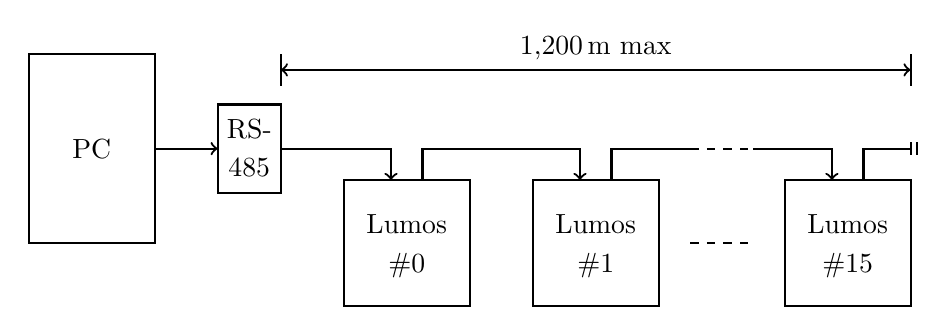
\begin{tikzpicture}[scale=.8]
		\draw [thick] (0,1) -- (0,4) -- (2,4) -- (2,1) -- cycle;
		\node at (1,2.5) {PC};
		\draw [thick] (3,1.8) -- (4,1.8) -- (4,3.2) -- (3,3.2) -- cycle;
		\node [above] at (3.5,2.5) {RS-};
		\node [below] at (3.5,2.5) {485};
		\foreach \x in {5, 8, 12} {
			\draw [thick] (\x, 0) -- (\x, 2) -- (\x+2, 2) -- (\x+2, 0) -- cycle;
			\node [above] at (\x+1, 1) {Lumos};
		};
		\node [below] at (6,1) {\#0};
		\node [below] at (9,1) {\#1};
		\node [below] at (13,1) {\#15};
		\draw [->, thick] (2,2.5) -- (3,2.5);
		\draw [->, thick] (4,2.5) -- (5.75,2.5) -- (5.75, 2);
		\draw [->, thick] (6.25,2) -- (6.25,2.5) -- (8.75,2.5) -- (8.75,2);
		\draw [thick]     (9.25,2) -- (9.25,2.5) -- (10.5,2.5);
		\draw [dashed, thick] (10.5, 2.5) -- (11.5,2.5);
		\draw [dashed, thick] (10.5, 1) -- (11.5, 1);
		\draw [->, thick] (11.5,2.5) -- (12.75, 2.5) -- (12.75, 2);
		\draw [thick]     (13.25, 2) -- (13.25, 2.5) -- (14, 2.5);
		\draw	[thick]   (14, 2.6) -- (14, 2.4);
		\draw	 [thick]  (14.1, 2.6) -- (14.1, 2.4);
		\draw   [thick]   (4, 4) -- (4, 3.5);
		\draw	[thick]   (14, 4) -- (14, 3.5);
		\draw [<->, thick] (4,3.75) -- (14, 3.75);
		\node [above] at (9, 3.75) {1,200\,m max};
	\end{tikzpicture}
	\caption{Network Connection Diagram\label{fig:net}}
\end{figure}

To connect the controllers to your PC, follow these steps:
\begin{enumerate}
	\item	Connect the \ix{\acronym*{RS-485} converter} to your PC's serial port using the serial cable
		which came with the converter unit.
	\item	Connect one end of an Ethernet-style cable to the \acronym{RS-485} converter.
	\item	The four-channel Lumos controller is designed to connect bare-wire ends of the communication
		cables to terminal block J1.  If connecting multiple Lumos boards directly to these
		terminal blocks, connect the incoming and outgoing segments of cable together to J1
		as shown in Figure~\ref{fig:wiring485cables}.
		If you are wiring a connector such as an 8-pin modular jack to the board, make sure to
		wire \emph{both} incoming and outgoing jacks to J1.  Do not connect them to each other
		with a single bit of cable from the jacks to J1.  %See Figure~\ref{fig:wiring485withjacks}.
	\item	Insert a 120\,$\Omega$ resistor pack R14 on the last Lumos board in the chain (as well as the first
		if the \acronym{PC} is connected in the middle of the chain), so that each end of the chain is
		terminated.
\end{enumerate}

\begin{figure}
	\centerfloat{\LLimg[height=2in]{4dc-485-single}\LLimg[height=2in]{4dc-485-dual}}
	\caption{Connected Network Cables: Single (left), Daisy-Chained (right)\label{fig:wiring485cables}}
\end{figure}
% wiring485cables
% wiring485withjacks

\section{Attaching Power Loads to the Lumos Controller}
The block of output channels is electrically isolated from the logic portion of the board, allowing them to have
separate power supplies in case the load is a different voltage than the logic supply.
You must supply power to the Lumos controller itself (at connector J6) as well as to the block of 
output channels you will be controlling at J7.

Also note that the Lumos output circuits were designed to control simple resistive loads such as
incandescent lights.  They are not appropriate for all kinds of loads.  Some inductive loads
(for example, electromagnetic relays and motors) may require a protective ``snubber'' circuit
which is not included in the Lumos product.  Adding snubber components to a Lumos board would be
a custom modification to the Lumos circuit and should not be attempted except by qualified engineers.

For these instructions, we will guide you through attaching an \mc{ATX}-style \ix{power supply} to a 
Lumos board, to supply +5\,V power to run the Lumos board itself, and +12\,V to run a string of \mc{RGB} \mc{LED}
Christmas lights.  Figure~\ref{fig:ledconn} shows how the wires are connected, using typical wire colors
employed by this style of power supply.

\begin{figure}
    \begin{center}
	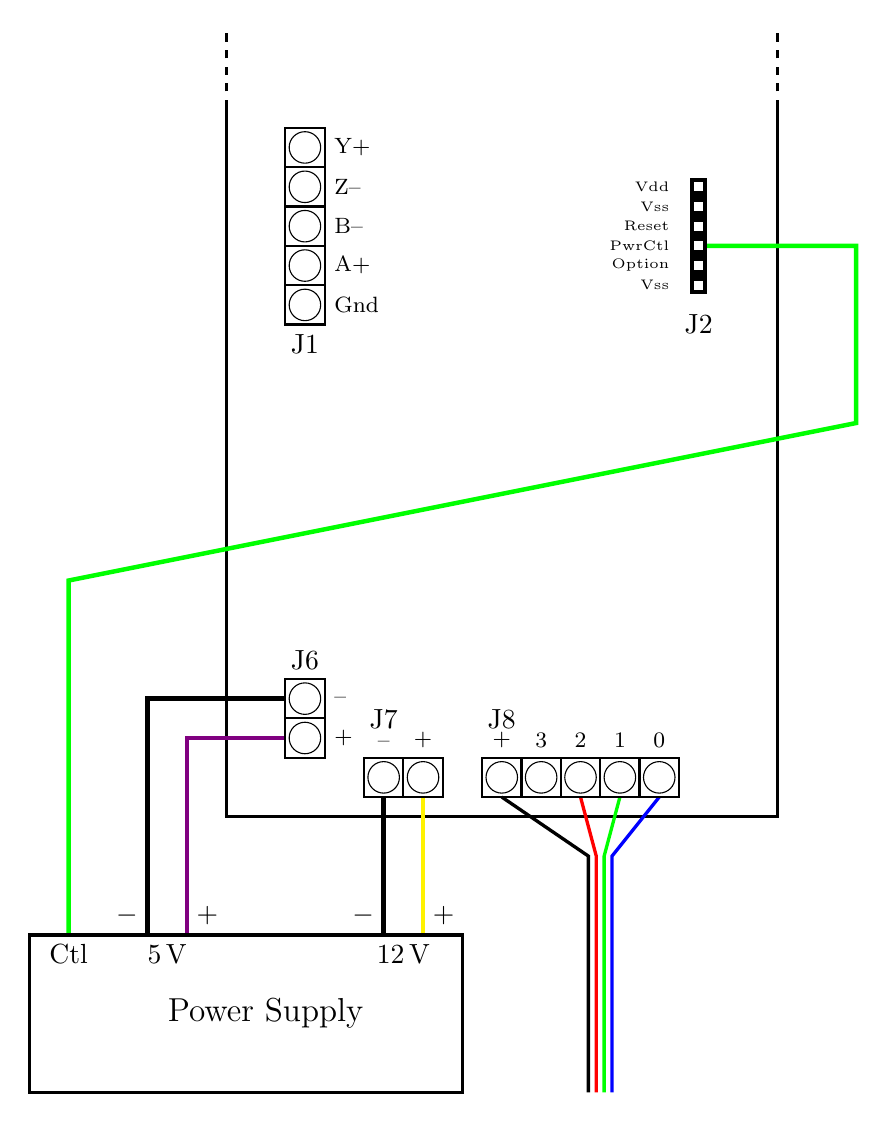
\begin{tikzpicture}
		\draw [very thick] (0,9) -- (0,0) -- (7,0) -- (7,9);
		\draw [very thick, dashed] (7,9) -- (7,10);
		\draw [very thick, dashed] (0,9) -- (0,10);

		\draw [ultra thick, black]  (-1.0,-1.5) -- (-1.0,1.5) -- (.75,1.5);
		\draw [ultra thick, violet] (-0.5,-1.5) -- (-0.5,1.0) -- (.75,1.0);
		\draw [ultra thick, black]  ( 2.0,-1.5) -- ( 2.0,.25);
		\draw [ultra thick, yellow] ( 2.5,-1.5) -- ( 2.5,.25);
		\draw [ultra thick, green]  (6,7.25) -- (8,7.25) -- (8,5) -- (-2,3) -- (-2,-1.5);

		\draw [very thick, black] (4.60, -3.5) -- (4.60, -.5) -- (3.50, .25);
		\draw [very thick, red]   (4.70, -3.5) -- (4.70, -.5) -- (4.50, .25);
		\draw [very thick, green] (4.80, -3.5) -- (4.80, -.5) -- (5.00, .25);
		\draw [very thick, blue]  (4.90, -3.5) -- (4.90, -.5) -- (5.50, .25);
		\node [above] at (3.5,1.0) {J8};
		\node [above] at (2,1.0) {J7};
		\foreach \x/\label in {2/--, 2.5/+, 3.5/+, 4/3, 4.5/2, 5/1, 5.5/0} {
			\foreach \y in {.5} {
				\draw [thick] (\x-.25,\y-.25)--(\x-.25,\y+.25)--(\x+.25,\y+.25)--(\x+.25,\y-.25)--cycle;
				\node [above] at (\x,\y+.25) {\footnotesize\label};
				\draw (\x,\y) circle (.2);
			}
		}
		\node [above] at (1,1.75) {J6};
		\foreach \x in {1} {
			\foreach \y/\label in {1/+, 1.5/--} {
				\draw [thick] (\x-.25,\y-.25)--(\x-.25,\y+.25)--(\x+.25,\y+.25)--(\x+.25,\y-.25)--cycle;
				\node [right] at (\x+.25,\y) {\footnotesize\label};
				\draw (\x,\y) circle (.2);
			}
		}
		\node [below] at (1,6.25) {J1};
		\foreach \x in {1} {
			\foreach \y/\label in {6.5/Gnd, 7/A+, 7.5/B--, 8/Z--, 8.5/Y+} {
				\draw [thick] (\x-.25,\y-.25)--(\x-.25,\y+.25)--(\x+.25,\y+.25)--(\x+.25,\y-.25)--cycle;
				\draw (\x,\y) circle (.2);
				\node [right] at (\x+.25,\y) {\footnotesize\label};
			}
		}
		\node [below] at (6,6.50) {J2};
		\draw[fill,black] (5.9,8.1) -- (6.1,8.1) -- (6.1, 6.65) -- (5.9, 6.65) -- cycle;
		\foreach \x in {6} {
			\foreach \y/\label in {8/Vdd, 7.75/Vss, 7.5/Reset, 7.25/PwrCtl, 7/Option, 6.75/Vss} {
				\draw [fill,white] (\x-.05,\y-.05)--(\x-.05,\y+.05)--(\x+.05,\y+.05)--(\x+.05,\y-.05)--cycle;
				\node [left] at (\x-.25,\y) {\tiny\label};
				%\draw (\x,\y) circle (.1);
			}
		}

		\node [below] at (-.75,-1.5) {5\,V};
		\node [above left] at (-1.0,-1.5) {$-$};
		\node [above right] at (-.5,-1.5) {$+$};
		\node at (.5,-2.5) {\large Power Supply};
		\node [above left] at (2,-1.5) {$-$};
		\node [above right] at (2.5,-1.5) {$+$};
		\node [below] at (2.25,-1.5) {12\,V};
		\node [below] at (-2,-1.5) {Ctl};
		\draw [very thick] (-2.5,-1.5) -- (3,-1.5) -- (3,-3.5) -- (-2.5,-3.5) -- cycle;
%
%		\draw [very thick, red]   (7.85, 0) -- (7.85, 3) -- (7.25, 4.5);
%		\draw [very thick, green] (7.95, 0) -- (7.95, 3) -- (7.75, 4.5);
%		\draw [very thick, blue]  (8.05, 0) -- (8.05, 3) -- (8.25, 4.5);
%		\draw [very thick, black] (8.15, 0) -- (8.15, 3) -- (8.75, 4.5);
%		\foreach \x in {5, 8} {
%			\foreach \y in {2, 1} {
%				\draw [fill, white] (\x, \y) circle (.4);
%				\draw [thick, black] (\x, \y) circle (.4);
%			}
%		};
%		\node at (6.5,1) {LED Strings};
	\end{tikzpicture}
	\caption{Example Wiring of a 12\,V R\mc{GB} L\mc{ED} String\label{fig:ledconn}}
    \end{center}
\end{figure}

{\bfseries Caution:}
The colors used here are typical for \acronym{ATX} power supplies, however
not all supplies use the same color codes to mark wires.  Connecting the wrong wires to the terminals
of the Lumos board may have catastrophic consequences, including serious injury, death, fire, and severe damage
\marginpar{\centerline{\LLimg[height=.5in]{danger-generic}}}
to the controller and all devices connected to it.  Check your power supply until you are \emph{certain} you know
exactly which wires carry which signals and voltages.  Be sure your power supply has the capacity to provide the
power needed for the loads you will plug into it and is appropriate for the environment where it will be used..

Make the main power connections to the board by following these steps:

\begin{enumerate}
	\item	Many \mc{ATX}-style power supplies have a wire which is used by the computer's motherboard
		to tell it when to start up or go to sleep (this is done to save power).  The Lumos
		board supports this feature.  If this power supply has such a wire, 
		connect it to pin~4 of header J2 using a matching wire-to-board connector.
		Typically, this is the {\bfseries green wire} from the power supply.  
%\newpage
	\item	We need to make sure the Lumos board is powered even if the power supply is in %``shutdown'' (also known as
		``sleep'' %) 
		mode.  The power supply provides a special +5\,V supply called the 
		``\ix{standby power}'' line,
		on a {\bfseries violet wire}.  Connect the violet wire to the ``+'' terminal of J6.

	\item	Connect a ground wire (typically {\bfseries black}) to the ``--'' terminal of J6.
		%\marginpar{\centerline{\LLimg[width=1.5in]{logic-pwr-connect-crop}}}

	\item\label{s:pwrjump}
		Configure the input voltage jumper J4.  If the board's logic circuits will be provided 
		with a regulated
		+5\,V DC supply to J6, place a single jumper across the middle pins of J4 (pins 2--3).  
		Otherwise, for input 
		supply voltages from +8\,V to +24\,V DC, place two jumpers on pins 1--2 and 3--4 of J4,
		as shown in Figure~\ref{fig:jumpers}.  In the example being described here, we are
		\marginpar{\centerline{\LLimg[width=1.5in]{4dc-j4-23}}}
		getting +5\,V so place a jumper across pins 2--3.
		\begin{description}
			\item[\HandRight\ Warning!]
				{\bfseries Be certain that the voltage select jumpers J3 and J4
				are correctly configured for the power you supply to the board.  If
				they are placed in the ``5\,V'' position but more than 5\,V is 
				supplied, it will destroy the Lumos board.}
			\item[\HandRight\ Advanced Tip:] 
				When the voltage select jumpers J3 and/or J4 
				are in the middle position
				(pins 2--3 shorted), the on-board voltage regulator is bypassed so the
				input power is sent directly into the circuit which is expecting +5\,V.
				This is necessary because the on-board +5\,V regulator needs at least
				+8\,V input to function.  If you select this, you must supply a clean,
				regulated +5\,V source.

				When the voltage select jumpers are in the other position (pins 1--2 are
				shorted together, and 3--4 are shorted together), the input power is routed
				through the on-board regulator.  The input voltage in this case must be
				between +8 and +24\,V~DC, but need not be perfectly regulated.
		\end{description}
\end{enumerate}

Attach loads to the Lumos board by connecting them to the output channel block. 
The output block is independently powered via its input power terminal block (J7).
When attaching power to this terminal, watch for the polarity as marked on the board.  The negative supply
is attached to the left terminal, while the positive terminal is on the right.

The four outputs are negative (--), and available at terminal block J8.
A common positive (+) output is also available there to power the controlled loads.

Follow these steps to attach the +12\,V light string for our example installation:

\begin{enumerate}
	\item 	Connect +12\,V to the block by attaching a {\bfseries yellow} wire from the power supply to
		the ``+'' (right) terminal of J7 on the Lumos board.

	\item	Attach another {\bfseries black} ground wire to the ``--'' (left) terminal of J7.
		%\marginpar{\centerline{\LLimg[width=1.5in]{block-12v-power}}}

	\item	Configure the block's input voltage by putting jumpers on J3 as described in 
		step~\ref{s:pwrjump} on page~\pageref{s:pwrjump}.  In this example, we're using +12\,V so we place
		two jumpers onto pins 1--2 and 3--4 of J3.
		\marginpar{\centerline{\LLimg[width=1.5in]{4dc-j4-1234}}}

	\item\label{s:led1}
		Attach the string of \mc{LED} lights by attaching its {\bfseries white} common wire to the ``+''
		terminal of J8.

	\item	Attach the light string's {\bfseries red} wire to the ``2'' terminal of J8.

	\item\label{s:led2}
		Repeat the previous step to attach the remaining color wires to terminals ``1'' and ``0'' on J8.

	\item	Plug the power supply into an AC outlet.
\end{enumerate}

\begin{figure}
    \begin{center}
	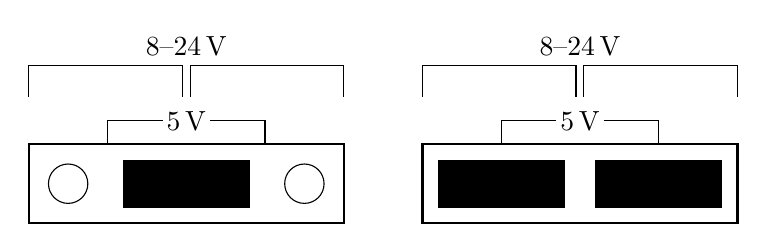
\begin{tikzpicture}
		\draw [thick] (0,0) -- (4,0) -- (4,1) -- (0,1) -- cycle;
		\draw (0.5,0.5) circle (.25);
		\draw (1.5,0.5) circle (.25);
		\draw (2.5,0.5) circle (.25);
		\draw (3.5,0.5) circle (.25);
		\draw (1,1) -- (1,1.3) -- (1.7,1.3);
		\draw (2.3,1.3) -- (3,1.3) -- (3,1);
		\node at (2,1.3) {5\,V};
		\draw (0,1.6) -- (0,2) -- (1.95,2) -- (1.95,1.6);
		\draw (2.05,1.6) -- (2.05,2) -- (4,2) -- (4,1.6);
		\node [above] at (2,2) {8--24\,V};
		\draw [fill] (1.2,0.2) -- (2.8,0.2) -- (2.8,0.8) -- (1.2,0.8) -- cycle;

		\draw [thick] (5,0) -- (9,0) -- (9,1) -- (5,1) -- cycle;
		\draw (6,1) -- (6,1.3) -- (6.7,1.3);
		\draw (7.3,1.3) -- (8,1.3) -- (8,1);
		\node at (7,1.3) {5\,V};
		\draw (5,1.6) -- (5,2) -- (6.95,2) -- (6.95,1.6);
		\draw (7.05,1.6) -- (7.05,2) -- (9,2) -- (9,1.6);
		\node [above] at (7,2) {8--24\,V};
		\draw [fill] (5.2,0.2) -- (6.8,0.2) -- (6.8,0.8) -- (5.2,0.8) -- cycle;
		\draw [fill] (7.2,0.2) -- (8.8,0.2) -- (8.8,0.8) -- (7.2,0.8) -- cycle;
	\end{tikzpicture}
	\caption{Input Voltage Select Jumpers for +5\,V (left) and +8--24\,V (right)\label{fig:jumpers}}
    \end{center}
\end{figure}

The board is now fully plugged in, connected, and ready to be controlled by the PC's software.

\section{Using a Common Supply}
If you wish to use a single power supply to power both the logic and controlled loads, simply attach
that supply to J7, and install jumpers onto J5 such that pins 1--2 and 3--4 are shorted.  Also be sure
that the voltage select jumpers J3 and J4 are correctly configured for the input voltage.

Note that if you do this, the loads and logic circuits will no longer be electrically isolated from
one another, but will all be part of one operating circuit.

\section{Checking Your Work}
You may test the connections you made before going all the way to the PC and running a sequencing program.
This verifies that everything is working and that the lights are plugged into the correct output channels.

\begin{enumerate}
	\item	Power on the board.
		{\bfseries Caution:} Exercise care when working with the live board.  Don't touch anything
		\marginpar{\centerline{\LLimg[height=.5in]{danger-sign}}}
		other than the jumper blocks as instructed here.  %(Unlike the Lumos AC relay boards, your Lumos DC board
		%should not normally have lethal voltages present on it, as it most often is used for small
		Even when used for low-voltage loads such as \mc{LED} lights, your application may involve
		hazardous current levels which may cause personal injury or death if not handled properly.

	\item	Check that the green \mc{LED} on the Lumos controller is slowly fading on and off.  This indicates
		that the controller is in its normal operating mode and is functioning correctly.

	\item	Insert a jumper onto pins 5--6 of J2 until the Lumos board's diagnostic lights all start
		flashing rapidly.
		\marginpar{\centerline{\LLimg[width=1.5in]{4dc-j2-56a}}}

	\item	Remove the jumper and wait a second or two for the lights to change to just the green light
		flashing rapidly (the others will be off).  
		The Lumos board is now in ``\ix{configuration mode}.''

	\item	Insert the jumper onto pins 5--6 again for at least 2~seconds.

	\item	Remove the jumper again.  The green light will turn off, and the red light will pulse rapidly.
		The Lumos board is now in ``\ix{field test mode}.''
\end{enumerate}

This mode is designed to help you check your connections before closing up the units and starting your
show.  The controller will cycle each output channel on for one second, then off again, starting with channel 0.  
Each second, the next channel in order from 0--3 will turn on, then will restart with channel 0 again.

When you're finished with this test, insert a jumper between pins 2--3 of J2 and then remove it again
to reset the controller back to normal operating mode.
\marginpar{\centerline{\LLimg[width=1.5in]{4dc-j2-23}}}

\begin{description}
	\item[\HandRight\ Tip:]  You can ``freeze'' the cycle, holding the currently-lit
		output channel on indefinitely, by inserting briefly and removing the jumper
		on pins 5--6 of J2.
		Insert and remove it again to resume the test cycle.
\end{description}

\chapter{Going On From Here}
Now that your controller is installed and ready to use, refer to the separate manual,
\emph{Using Lumos SSR Controllers} for full instructions on how to program
and use your controller with your computer or in stand-alone operation.

%\section{Getting Additional Help}
The \ix{product website} at \URL{www.alchemy.com/lumos} contains additional documentation,
\index{website}
pointers, hints, and tips to assist you further.  If that doesn't answer all your questions,
there is an \ix{online forum} where you may submit questions for help.

\backmatter
\appendix

\input 4pinouts

\chapter{Troubleshooting}\label{ch:troubleshooting}
%\LLstart{W}{HILE}{we anticipate} 
While we anticipate the Lumos board will provide many hours of worry-free operation,
as with any device (particularly one built as a \acronym{DIY} project), sometimes things don't go
quite as planned.  Here are a few common problems and their solutions.

\begin{longtable}{|p{1.5in}|p{1.5in}|p{2in}|}\hline
\bfseries Symptom & \bfseries Likely Cause(s) & \bfseries Solution \\\hline\hline
\endhead
The entire block of outputs does not turn on 
	& No power to the block 
	& Check the fuse,
	  the connection from the power supply to the block, and that the power supply is powered on.\\
\cline{2-3}
	& Power supply not told to wake up (\mc{ATX}-style supplies only).
	& Check that the power supply's green wire is attached to the $\overline{\hbox{\mc{PWR CTL}}}$
	  output (J2, pin~4). \\\hline
Some outputs don't work, or are erratic.
	& Loose % opto-isolator 
chip.
	& Lightly press chip U3 back into its socket.\\
\cline{2-3}
	& Bad solder connection or loose chip.
	& Re-check all solder connections on the board, re-solder any which are cold, broken, or
	  incomplete.\\\hline
No units in serial network respond to commands.
	& Missing terminator
	& Replace terminators on both ends of the daisy chain (note the PC's RS485 converter
	  may include a built-in terminator for that position).\\\hline
One unit does not respond to commands.
	& Wrong address.
	& Use the \verb+lumosctl+ program to reconfigure the board to have
	  the correct address.\\\hline
\end{longtable}


%\chapter{Diagnostics}\label{ch:diagnostics}


\chapter{Glossary}\label{ch:glossary}
\begin{description}
	\item[Active High:]
		A logic signal which is considered ``on'' when the signal is ``high'' (binary 1 or +5\,V),
		and ``off'' when the signal is ``low'' (binary 0 or 0\,V).  Lumos relay circuits are 
		triggered with active-low signals.
	\item[Active Low:]
		A logic signal which is considered ``on'' and ``off'' at the opposite signal levels
		to an ``active high'' signal (q.v.).
%	\item[Annular Ring:]
%		The exposed ring of metal around a hole in a \acronym{PCB} where a component is to be 
%		mounted.  The solder will flow across the component lead and onto the annular ring.
	\item[Daisy Chain:]
		The arrangement of wiring a number of devices together by connecting the first to the second,
		then adding another connection from the second to the third, and so forth.  The network
		connection diagram in Figure~\ref{fig:net} shows an example of a daisy chain.
%	\item[\acronym{DIP} (Dual In-line Package):]
%		The style of chip where the pins are laid out in two parallel rows.
	\item[\acronym{DCE} (Data Communications Equipment):]  In the realm of \acronym{RS-232} devices, this is the peripheral
		device plugged into the main ``terminal'' (\acronym{DTE}) device.  Examples include
		Lumos controllers and modems.
	\item[\acronym{DIY}:] ``Do-It-Yourself.''
	\item[\acronym{DTE} (Data Terminal Equipment):]  In the realm of \acronym{RS-232} devices, this is the
		main ``terminal'' device such as a PC or teletype.
	\item[Duplex:]
		a feature of a serial line.  On a full-duplex connection, separate data wires are present
		to carry data in both directions, so one device can send and receive data at the same time.
		On a half-duplex connection, only a single set of data wires is present, so devices must
		take turns transmitting over them.
	\item[\acronym{ESD} (Electro-Static Discharge):]
		static electricity which builds on your skin and is then discharged into sensitive
		components when you touch them.  Invisible to the eye, this can punch microscopic holes
		in the inside of the components, severely damaging them.
%	\item[Heat Protection:]
%		A temporary heat sink applied to a component when soldering that component onto
%		the \acronym{PCB}.  Typically used for heat-sens\-i\-tive components such as transistors
%		and integrated circuit chips.
	\item[Jumper Block:]
		A series of pins mounted to the \acronym{PCB}.  Different options are configured for the
		circuit by placing a jumper over certain pairs of pins, shorting them together.
	\item[\acronym{LED} (Light Emitting Diode):]
		A special kind of diode which emits light when current passes from its anode to its cathode.
%	\item[\acronym{MOSFET}:]
%		The type of transistor which forms the major part of a Lumos DC relay channel.  The name
%		is an acronym for Metal Oxide Semiconductor Field Effect Transistor.
	\item[\acronym{PCB} (Printed Circuit Board):]
		The board where electronic components are mounted to form a complete circuit.  Metal
		traces are ``printed'' (actually etched) onto the surface of the board itself to make the
		connections between components.
	\item[RS-485:]
		A standard hardware protocol for sending serial data between multiple devices on a single
		cable length (electrically it is a single cable which each device ``taps into'' along the
		line; physically it is typically a ``daisy chain'' arrangement where a short cable connects
		one device to the next, another cable to the next, and so on). Unshielded twisted-pair cable
		is used (like Ethernet cable), and the cable lengths should not exceed a total of 4,000\,ft
		(1,200\,m).
	\item[Terminator Plug:]
		An \acronym{RS-485} network requires a terminator at each end.  This is a small plug which plugs into
		the last unit in the daisy chain.
	\item[\acronym{TTL} (Transistor-Transistor Logic):] One of the ways digital logic circuits can be
		constructed.  For our purposes here, we consider a ``\acronym{TTL}-level'' signal to be a
		logic input or output where a voltage near +5\,V is ``high'' (binary 1 or ``true'') and a
		voltage near 0\,V is ``low'' (binary 0 or ``false'').  The inputs should never be above
		+5 nor below 0 volts.
\end{description}

\input acknowledgements 

\indexintoc
\printindex
\clearpage

\input colophon
\end{document}
